\Opensolutionfile{ans}[ans/ansTL-CD6]
\setcounter{ex}{0}
\subsubsection{Đề số 3}

\begin{ex}%[0D1Y1]
	Câu nào sau đây \textbf{không} phải là mệnh đề.
	\choice
	{$3+4 \ge 8$}
	{\True $ 2+x=3$}
	{$3-2=1$}
	{$2<\sqrt 3$}
	\loigiai{
	}
\end{ex}

\begin{ex}%[0D1Y1-3]
	Mệnh đề phủ định của mệnh đề \lq \lq $2018$ là số tự nhiên chẵn\rq \rq \, là
	\choice
	{$ 2018 $ là số chẵn}
	{\True $ 2018 $ không là số tự nhiên chẵn}
	{$ 2018 $ là số nguyên tố}
	{$ 2018 $ là số chính phương}
	\loigiai{
		Phủ định của mệnh đề đã cho là \lq \lq $2018$ không là số tự nhiên chẵn\rq \rq .
	}
\end{ex}

\begin{ex}%[0D1Y3-1]
	Cho hai tập hợp $E=(-\infty;6]$ và $F=[-2;7]$. Khi đó $E\cap F$ là
	\choice
	{\True $E\cap F = [-2;6]$}
	{$E\cap F = (-\infty;7]$}
	{$E\cap F = (-\infty;-2)$}
	{$E\cap F = [6;7]$}
	\loigiai{
		\immini{
			Ta có $E \cap F=[-2;6]$.}
		{\vspace{-0.5cm}
			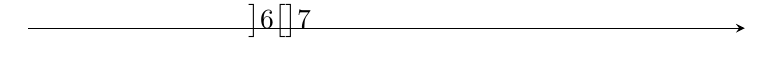
\begin{tikzpicture}[scale=0.7,>=stealth]
			\draw[->](-4,0)->(9,0);%Vẽ trục số
			\def\skipInterval{0.5cm}%Khoảng cách đặt nhãn
			\def\colorInterval{blue} %Màu tick, màu fill miền
			\IntervalLR{6}{9}\IntervalGLF{\big]}{$6$}{}{}
			\IntervalLR{-4}{-2}
			\IntervalGRF{}{}{\big[}{-2}
			\IntervalLR{7}{9}
			\IntervalGRF{\big]}{$7$}{}{}
			\end{tikzpicture}}
	}
\end{ex}

\begin{ex}%[0D1Y4-1]
	Tập hợp $X=(-\infty;2] \cap (-6;+\infty)$ là
	\choice
	{$(-4;9]$}
	{$\mathbb{R}$}
	{$(-6;2]$}
	{\True $[-6;2]$}
	\loigiai{
		Ta có: $X=(-6;2]$.}
\end{ex}

\begin{ex}% [Chuyên Lương Thế Vinh - Đồng nai 2018]%[0D1B3]
	\immini[thm]{Cho các tập hợp $ A$, $B $ được minh họa bằng biểu đồ Ven như hình bên. Phần tô màu xám trong hình là biểu diễn của tập hợp nào sau đây?
		\haicot
		{$A \cup B$}
		{$A \cap B$}
		{\True $A \backslash B$}
		{$B \backslash A$}
	}
	{
		\begin{venndiagram2sets}[tikzoptions={scale=0.7,thick}]
			\fillANotB
	\end{venndiagram2sets}}	
\loigiai{
}
\end{ex}

\begin{ex}%[0D1B3]
	Cho ba tập hợp $A=\{1; 2; 3; 4; 5; 6; 9\}$, $B=\{0; 2; 4; 6; 8; 9\}$, $C=\{3; 4; 5; 6; 7\}$. Tính tích các phần tử của tập hợp $A \cap (B \backslash C)$.
	\choice
	{\True $18$}
	{$7$}
	{$11$}
	{$2$}
	\loigiai{
	}
\end{ex}

\begin{ex}%[0D1B1]
	Trong các câu sau, có bao nhiêu câu là mệnh đề?
	\begin{listEX}[2]
		\item [(1)]\quad Hãy mở cửa ra!
		\item [(2)]\quad Số 20 chia hết cho 8.
		\item [(3)] \quad Số 17 là một số nguyên tố.
		\item [(4)] \quad Bạn có thích chơi bóng đá không?
	\end{listEX}
	\choice
	{\True $2$}
	{$4$}
	{$3$}
	{$1$}
	\loigiai{
	}
\end{ex}


\begin{ex}%[0D1B2]
	Tập hợp $A=\left\{x\in \mathbb{R}\big| 2x^2-7x+1=0\right\}$ có bao nhiêu phần tử?
	\choice
	{\True $2$}
	{$1$}
	{vô số}
	{$0$}
	\loigiai{
		Xét phương trình $2x^2-7x+1=0$ luôn có hai nghiệm thực phân biệt nên tập $A$ có hai phần tử.
	}
\end{ex}

\begin{ex}%[0D1B1-2]
	Trong các mệnh đề sau, mệnh đề nào là mệnh đề \textbf{sai}?
	\choice
	{$\pi <4 \Leftrightarrow \pi^2<16$}
	{$\sqrt{23}<5 \Rightarrow -2\sqrt{23}>-2 \cdot 5$}
	{\True $-\pi <-2 \Leftrightarrow \pi^2<4$}
	{$\sqrt{23}<5 \Rightarrow 2\sqrt{23}<2 \cdot 5$}
	\loigiai{
		Ta có $-\pi <-2 \Rightarrow \pi^2>4$. Suy ra A sai.\\
		Có $\pi <4 \Leftrightarrow \pi^2<16$; $\sqrt{23}<5 \Rightarrow 2\sqrt{23}<2 \cdot 5$;$\sqrt{23}<5 \Rightarrow -2\sqrt{23}>-2 \cdot 5$ luôn đúng.}
\end{ex}

\begin{ex}%[0D1B3]
	Cho hai tập hợp $X=\left\{0, 1, 2, 3, 4\right\}$ và $Y=\left\{ 2, 3, 4, 5, 6 \right\}$. Tìm tập hợp $X\setminus Y$.
	\choice
	{$\left\{ 1, 2 \right\}$}
	{$\left\{ 1, 5 \right\}$}
	{\True $\left\{ 0, 1 \right\}$}
	{$\left\{ 0 \right\}$}
	\loigiai{
	}
\end{ex}

\begin{ex}
	Kết quả của phép toán $\mathbb{R}\backslash [-1;2)$ được minh họa lên trục số là hình nào sau đây?
	\choice
	{\begin{tikzpicture}[>=stealth]
		\draw[->](-1,0)--(5,0)node[below]{$+\infty$};
		\IntervalLR{-1}{1/2}
		\def\skipInterval{0.5cm}%Khoảng cách đặt nhãn
		\IntervalGRF{}{}{\big[}{2}%Gạch xọc phải qua trái
		\IntervalLR{4}{4.8}
		\def\skipInterval{0.5cm}%Khoảng cách đặt nhãn
		%\IntervalGRF{\big]}{b}{}{}%Gạch xọc phải qua trái
		\end{tikzpicture}}
	{\True 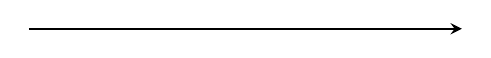
\begin{tikzpicture}[xscale=0.5,thick,>=stealth]
		\draw[->](-5,0)->(6,0);
		\IntervalRF{)}{-1}{[}{2}
		\end{tikzpicture}}
	{\begin{tikzpicture}[>=stealth]
		\draw[->](-1,0)node[below]{$-\infty$}--(5,0);
		\IntervalLR{-1}{1/2}
		\def\skipInterval{0.5cm}%Khoảng cách đặt nhãn
		%\IntervalGRF{}{}{\big[}{a}%Gạch xọc phải qua trái
		\IntervalLR{3}{4.8}
		\def\skipInterval{0.5cm}%Khoảng cách đặt nhãn
		\IntervalGRF{\big)}{-1}{}{}%Gạch xọc phải qua trái
		\end{tikzpicture}}
	{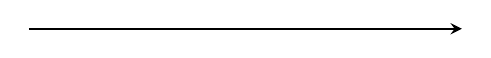
\begin{tikzpicture}[xscale=0.5,thick,>=stealth]
		\draw[->](-5,0)->(6,0);
		\IntervalRF{]}{-1}{(}{2}
		\end{tikzpicture}}
	\loigiai{
		Ta có $\mathbb{R}\backslash [-1;2)=(-\infty;-1) \cup [2;+\infty]$. 
	}
\end{ex}
\begin{ex}%[0D1B2-1]
	Tập $S=\left\{q \in \mathbb{Q}|\; 25q^4-9q^2=0\right\}$ có bao nhiêu phần tử?
	\choice
	{$1$}
	{$4$}
	{\True $3$}
	{$2$}
	\loigiai{
		Ta có $25q^4-9q^2=0 \Leftrightarrow \hoac{&q=0 \in \mathbb{Q} \\& q=\pm \dfrac{3}{5} \in \mathbb{Q}}$ nên $S=\left\{0;-\dfrac{3}{5};\dfrac{3}{5}\right\}$.}
\end{ex}

\begin{ex}%[0D1B2]
	Cho $E$ là tập hợp các hình tứ giác; $F$ là tập hợp các hình thang; $G$ là tập hợp các hình thoi. Trong các mệnh đề sau, mệnh đề nào \textbf{sai}?
	\choice
	{$G\subset E$}
	{$F\subset E$}
	{$G\subset F$}
	{\True $E\subset G$}
	\loigiai{
	Ta có hình thoi là một tứ giác nên $G\subset E$. Suy ra khẳng định $E\subset G$ là khẳng định sai.
	}
\end{ex}

\begin{ex}%[0D1B3-1]
	Cho $A=\{1;5\}$, $B=\{1;3;5\}$. Chọn kết quả đúng trong các kết quả sau.
	\choice
	{$A \cup B=\{3;5\}$}
	{$A \cup B=\{1;3\}$}
	{$A \cap B=\{1\}$}
	{\True $A \cap B=\{1;5\}$}
	\loigiai{
		Ta có $A \cap B=\{1;5\}$.}
\end{ex}

\begin{ex}%[0D1B1]
	Phủ định của mệnh đề  $\exists x\in\mathbb{Z}:1-x^2\geq 0$ là
	\choice
	{$\forall x\in\mathbb{Z}:1-x^2\geq 0$}
	{$\exists x\in\mathbb{Z}:1-x^2< 0$}
	{$\forall x\in\mathbb{Z}:1-x^2\neq 0$}
	{\True $\forall x\in\mathbb{Z}:1-x^2<0$}
	\loigiai{
	}
\end{ex}

\begin{ex}%[0D1K3]
	Cho hai tập hợp $A=\left\{ x\in \mathbb{R}\big| x+2\geq 0 \right\}$ và $B=\left\{ x\in \mathbb{R}\big| 5-x\geq 0 \right\}$. Tìm tập hợp $A \setminus B$.
	\choice
	{\True $\left( 5;+\infty  \right)$}
	{$\left( 2;+\infty  \right)$}
	{$\left[ -2;6 \right]$}
	{$\left[ -2;5 \right]$}
	\loigiai{
		Ta có
		\begin{itemize}
			\item [$\bullet$] $x+2 \ge 0 \Leftrightarrow x \ge -2$ và $x \in \mathbb{R}$ nên $A=[-2;+\infty)$.
			\item [$\bullet$] $5-x \ge 0 \Leftrightarrow x \le 5$ và $x \in \mathbb{R}$ nên $B=(-\infty;5]$.
		\end{itemize} 
		Suy ra $A \setminus B= \left( 5;+\infty  \right)$.
	}
\end{ex}

\begin{ex}%[0D1K4]
	Cho tập hợp $A=\left(0;1\right)$. Hãy xác định tập hợp $\mathrm{C}_{\mathbb{R}}A.$
	\choice
	{\True$\mathrm{C}_{\mathbb{R}}A=\left(-\infty;0\right]\cup\left[1;+\infty\right)$}
	{$\mathrm{C}_{\mathbb{R}}A=\left(-\infty;0\right]\cup\left(1;+\infty\right)$}
	{$\mathrm{C}_{\mathbb{R}}A=\left(-\infty;0\right)\cup\left[1;+\infty\right)$}
	{$\mathrm{C}_{\mathbb{R}}A=\left(-\infty;0\right)\cup\left(1;+\infty\right)$}
	\loigiai{
	}
\end{ex}

\begin{ex}%[Đào Trung Kiên]%[0D1K2]
	Tập hợp $\left\{1; 2; 3\right\}$ có bao nhiêu tập con?
	\choice
	{$6$}
	{$7$}
	{$3$}
	{\True $8$}
	\loigiai{
		Tập $A$ có 3 phần tử nên số tập con của $A$ là $2^3=8$ tập.
	}
\end{ex}

\begin{ex}%[0D1K1]
	Mệnh đề nào là mệnh đề \textbf{sai}?
	\choice
	{Tứ giác $ABCD$ nội tiếp đường tròn tâm $O\Leftrightarrow OA=OB=OC=OD$}
	{$\triangle ABC $ đều $\Leftrightarrow \triangle ABC$ cân và có $1$ góc bằng $60^\circ$ }
	{Tam giác $ABC$ vuông tại $C$ $\Leftrightarrow AB^2=AC^2+CB^2$}
	{\True Một $\triangle ABC$ đều thì $\triangle ABC$ cân và ngược lại }
	\loigiai{}
\end{ex}

\begin{ex}%[0D1K4]
	Cho hai tập hợp $A=\lbrace x \in \mathbb{N}\big| x+3<4+2x \rbrace$ và $B= \lbrace x \in \mathbb{R} \big| 5x-3 < 4x-1  \rbrace$. Tất cả các số tự nhiên thuộc cả hai tập hợp $A$ và $B$ là
	\choice
	{$-2$ và $2$}
	{$-3$ và $-2$}
	{\True $0$ và $1$}
	{$-1$ và $1$}
	\loigiai{
		\begin{itemize}
			\item [$\bullet$] $x+3<4+2x \Leftrightarrow x>-1$.
			\item [$\bullet$] $5x-3 < 4x-1 \Leftrightarrow x<2$
		\end{itemize} 
	Các số tự nhiên thuộc cả hai tập hợp $A$ và $B$ chính là các số tự nhiên $x$ thỏa $-1<x<2$ nên $x \in \{0;1\}$.
	}
\end{ex}

\begin{ex}%[0D1G3]
	Xét các tập hợp $X, Y$ có cùng số phần tử. Biết rằng số phần tử của tập hợp $X \cup Y$ và $C_XY$ lần lượt là 35 và 15. Tìm số phần tử của tập hợp $X$.
	\choice
	{$35$}
	{\True $20$}
	{$50$}
	{$15$}
	\loigiai{
		Có 15 phần tử của tập $X$ không phải là phần tử của tập $Y$ nên số phần tử của tập hợp $X \cup Y$ bằng số phần tử sẵn có của $Y$ cộng thêm số phần tử thuộc tập $C_XY$. Do đó, tập $X$ và tập $Y$ cùng có 20 phần tử.
	} 
\end{ex}

\begin{ex}%[0D1B3-2]
	Cho các tập hợp $A=[m;m+2]$, $B=[-1;2]$. Điều kiện của $m$ để $A \subset B$ là
	\choice
	{$\hoac{&m \leq 1 \\& m \geq 0}$}
	{$\hoac{&m<-1 \\& m>2}$}
	{\True $-1 \leq m \leq 0$}
	{$1 \leq m \leq 2$}
	\loigiai{
		$A \subset B \Leftrightarrow \heva{&-1 \leq m \\& m+2 \leq 2}\Leftrightarrow \heva{&m \geq -1 \\& m \leq 0}\Leftrightarrow -1 \leq m \leq 0$.}
\end{ex}

\begin{ex}%[0D1B4-1]
	Cho các tập hợp $A=(1-2m;m+1],B=(-3;5)$. Tất cả các giá trị của $m$ sao cho $B$ là tập con của $A$ là
	\choice
	{$m \leq 4$}
	{\True $m \geq 4$}
	{$m \leq 2$}
	{$m \geq 2$}
	\loigiai{
		Điều kiện $1-2m<m+1\Leftrightarrow m>0$.\\
		Để tập $B$ là tập con của $A$ thì $\heva{&1-2m \leq 3 \\& m+1 \geq 5}\Leftrightarrow \heva{&m \geq -1 \\& m \geq 4}\Leftrightarrow m \geq 4$.}
\end{ex}

\begin{ex}%[0D1B4-1]
	Cho hai tập hợp khác rỗng $A=(m-1;4]$ và $B=(-2;2m+2)$, với $m\in \mathbb{R}$. Tìm $m$ để $A\cap B \ne \varnothing$.
	\choice
	{$m<5$}
	{$-3<m<5$}
	{\True $-2<m<5$}
	{$-3<m$}
	\loigiai{
		Hai tập $A$, $B$ khác rỗng $\Leftrightarrow  \heva{& m-1 < 4\\& 2m+2 > -2} \Leftrightarrow -2 < m< 5. \hfill (1)$\\
		Ta có $A\cap B = \varnothing \Leftrightarrow 2m+2 \le m-1 \Leftrightarrow m\le -3. \hfill (2)$\\
		Từ $(1)$ và $(2)$ suy ra $A\cap B \ne \varnothing \Leftrightarrow -2 < m < 5$.
	}
\end{ex}

\begin{ex}%[PHAN HIEU - TLDH5]%[0D1G3-3]%
	Lớp 10B1 có $ 7$ học sinh giỏi Toán, $ 5$ học sinh giỏi Lý, $ 6$ học sinh giỏi Hóa,
	$ 3$ học sinh giỏi cả Toán và Lý, $ 4$ học sinh giỏi cả Toán và Hóa, $ 2$ học sinh giỏi cả Lý và Hóa, $ 1$ học sinh giỏi cả $ 3$ môn Toán, Lý, Hóa. Số học sinh giỏi ít nhất một môn (Toán, Lý, Hóa) của lớp 10B1 là
	\choice
	{\True $ 10$}
	{$28$}
	{$18$}
	{$9$}
	\loigiai{
		Ta dùng biểu đồ Ven để giải\\
		\begin{center}
			\begin{tikzpicture}
				\begin{scope}[line join=round,thick,fill opacity=0.4]
					\fill[red] (0,0) circle (1.5cm);
					\fill[green] (20:2cm) circle (1.6cm);
					\fill[blue] (-35:1.7cm) circle (1.4cm);
				\end{scope}
				\draw[blue] (0,0) circle (1.5cm);
				\draw[blue] (20:2cm) circle (1.6cm);
				\draw[blue] (-35:1.7cm) circle (1.4cm);
				\path (-.5,0)node{$ 1 $} (-5:1.05)node{$ 1 $} (-10:2)node{$ 1 $}
				(-55:1)node{$ 3 $} (-45:2.2)node{$ 1 $}
				(45:1.05)node{$ 2 $} (25:2.5)node{$ 1 $};
				\draw[stealth-stealth] (-65:1)--(-2,-2)node[below]{Giỏi Toán + Hóa}--(-10:.8);
				\draw[stealth-stealth] (35:1.3)--(1.1,2.5)node[above]{Giỏi Toán + Lý}--(5:.8);
				\draw[stealth-stealth] (-10:2.4)--(4,0)node[right]{Giỏi Lý + Hóa}--(0:1.3);
				\draw[-stealth] (-2.5,2)node[above]{Toán}--(135:1.5);
				\draw[-stealth] (4.5,2)node[right]{Lý}--($ (20:2)+(30:1.6) $);
				\draw[-stealth] (4.5,-2)node[right] {Hóa}--($ (-35:1.7)+(-30:1.4) $);
			\end{tikzpicture}
		\end{center}
		Số học sinh giỏi Toán, Lý mà không giỏi Hóa: $ 3-1=2$.\\
		Số học sinh giỏi Toán, Hóa mà không giỏi Lý: $ 4-1=3$.\\
		Số học sinh giỏi Hóa, Lý mà không giỏi Toán: $ 2-1=1$.\\
		Số học sinh chỉ giỏi môn Lý: $ 5-2-1-1=1$.\\
		Số học sinh chỉ giỏi môn Hóa: $ 6-3-1-1=1$.\\
		Số học sinh chỉ giỏi môn Toán: $ 7-3-2-1=1$.\\
		Số học sinh giỏi ít nhất một (môn Toán, Lý, Hóa) là số học sinh giỏi $ 1$ môn hoặc $ 2$ môn hoặc cả $ 3$ môn: $ 1+1+1+1+2+3+1=10$.
	}
\end{ex}
\centerline{\textbf{---HẾT---}}
\Closesolutionfile{ans}
